\documentclass{standalone}
\usepackage{tikz}
\usetikzlibrary{arrows,decorations.markings,calc,positioning}
\begin{document}%
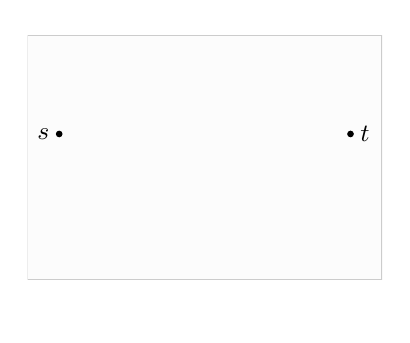
\begin{tikzpicture}[font=\small]

\ifdefined\argstonly
\fi

\ifdefined\argstexisting
   \def\drawexisting{}
\fi

\ifdefined\argtarget
   \def\drawexisting{}
   \def\drawtarget{}
\fi

\ifdefined\argotherpaths
   \def\drawexisting{}
   \def\drawtarget{}
   \def\drawotherpaths{}
\fi

\ifdefined\argall
   \def\drawexisting{}
   \def\drawtarget{}
   \def\drawotherpaths{}
   \def\drawcandidate{}
\fi

\clip (0,-0.45) rectangle (4.5,3.2);

\begin{scope}
\clip (0,0.0) rectangle (4.5,3.1);
\draw[black!20,fill=black!1] (0,0.0) rectangle (4.5,3.1);
%\draw[step=0.5cm,gray,very thin] (0,0) grid (4.5,3.5);

% start
\coordinate (s) at (0.4,1.85);

% goal
\coordinate (g) at (4.1,1.85);

% sample #1
\coordinate (q1) at (1.8,3.3);

% from start tree
\coordinate (q1sn) at (s);
\coordinate (q1sr) at ($(q1sn)!0.6!(q1)$);

% from goal tree
\coordinate (q1gn) at (g);
\coordinate (q1gr) at ($(q1gn)!0.7!(q1)$);

% sample #2
\coordinate (q2) at (2.0,1.6);

% from start tree (from midpoint down to q2)
\coordinate (q2sn) at ($(q1sn)!(q2)!(q1sr)$);
\coordinate (q2sr) at ($(q2sn)!0.6!(q2)$);

% from goal tree (from midpoint down to q2)
\coordinate (q2gn) at ($(q1gn)!(q2)!(q1gr)$);
\coordinate (q2gr) at ($(q2gn)!0.5!(q2)$);

% sample #3
\coordinate (q3) at (2.7,0.6);

% no extension from start

% from goal tree (from end of q2gr)
\coordinate (q3gn) at (q2gr);
\coordinate (q3gr) at ($(q3gn)!0.4!(q3)$);

% sample #4
\coordinate (q4) at (0.5,2.6);

\coordinate (q4sn) at ($(q1sn)!(q4)!(q1sr)$);
\coordinate (q4sr) at (q4);

% no extension from goal

% sample #5
\coordinate (q5) at (3.5,2.9);

% no extension from start

% from goal tree
\coordinate (q5gn) at ($(q1gn)!(q5)!(q1gr)$);
\coordinate (q5gr) at (q5);

% sample #6
\coordinate (q6) at (1.5,0.5);

% from start tree
\coordinate (q6sn) at (q2sr);
\coordinate (q6sr) at (q6);

% from goal tree
\coordinate (q6gn) at (q3gr);
\coordinate (q6gr) at ($(q6gn)!0.4!(q6)$);

% sample #7
\coordinate (q7) at (1.2,1.6);

% from start tree
\coordinate (q7sn) at ($(q6sn)!(q7)!(q6sr)$);
\coordinate (q7sr) at (q7);

% from goal tree
\coordinate (q7gn) at ($(q3gn)!(q7)!(q3gr)$);
\coordinate (q7gr) at ($(q7gn)!0.2!(q7)$);

% sample #7
\coordinate (q8) at (3.5,1.6);

% from start tree
\coordinate (q8sn) at ($(q6sn)!(q8)!(q6sr)$);
\coordinate (q8sr) at ($(q8sn)!0.05!(q8)$);

% from goal tree
\coordinate (q8gn) at ($(q1gn)!(q8)!(q1gr)$);
\coordinate (q8gr) at (q8);

% sample #9
\coordinate (q9) at (3.0,0.6);

% from start tree
\coordinate (q9sn) at ($(q6sn)!(q9)!(q6sr)$);

% from goal tree
\coordinate (q9gn) at ($(q6gn)!(q9)!(q6gr)$);

%\node[circle,fill=blue!30,inner sep=0.0cm] at (q1) {\tiny 1};
%\node[circle,fill=blue!30,inner sep=0.0cm] at (q2) {\tiny 2};
%\node[circle,fill=blue!30,inner sep=0.0cm] at (q3) {\tiny 3};
%\node[circle,fill=blue!30,inner sep=0.0cm] at (q4) {\tiny 4};
%\node[circle,fill=blue!30,inner sep=0.0cm] at (q5) {\tiny 5};
%\node[circle,fill=blue!30,inner sep=0.0cm] at (q6) {\tiny 6};
%\node[circle,fill=blue!30,inner sep=0.0cm] at (q7) {\tiny 7};
%\node[circle,fill=blue!30,inner sep=0.0cm] at (q8) {\tiny 8};
%\node[circle,fill=blue!30,inner sep=0.0cm] at (q9) {\tiny 9};

\ifdefined\drawexisting

% rrt lines
\draw[black!20,line width=3pt,line cap=round] (q1sn) -- (q1sr);
\draw[black!20,line width=3pt,line cap=round] (q1gn) -- (q1gr);
\draw[black!20,line width=3pt,line cap=round] (q2sn) -- (q2sr);
\draw[black!20,line width=3pt,line cap=round] (q2gn) -- (q2gr);
\draw[black!20,line width=3pt,line cap=round] (q3gn) -- (q3gr);
\draw[black!20,line width=3pt,line cap=round] (q4sn) -- (q4sr);
\draw[black!20,line width=3pt,line cap=round] (q5gn) -- (q5gr);
\draw[black!20,line width=3pt,line cap=round] (q6sn) -- (q6sr);
\draw[black!20,line width=3pt,line cap=round] (q6gn) -- (q6gr);
\draw[black!20,line width=3pt,line cap=round] (q7sn) -- (q7sr);
\draw[black!20,line width=3pt,line cap=round] (q7gn) -- (q7gr);
\draw[black!20,line width=3pt,line cap=round] (q8sn) -- (q8sr);
\draw[black!20,line width=3pt,line cap=round] (q8gn) -- (q8gr);

\fi

% draw start/goal/last query
\node[circle,fill=black,inner sep=0.03cm] at (s) {};
\node[left=0.0cm of s] {$s$};
\node[circle,fill=black,inner sep=0.03cm] at (g) {};
\node[right=0.0cm of g] {$t$};

\ifdefined\drawtarget
\node[circle,fill=black!30,inner sep=0.03cm] at (q9) {};
\node[below right=-0.1cm of q9] {$q_i$};
\fi

\ifdefined\drawotherpaths
% candidate paths
% straight lines
\draw[black!50,line width=1pt,densely dotted] (s) -- (q9) -- (g);
% wavy
\draw[black!50,line width=1pt,densely dotted]
   (s) .. controls (0.8,-0.4) and (2.9,0.1) .. (q9)
   .. controls (3.1,1.1) and (3.0,1.85) .. (g);
% other path through trees
\draw[black!50,line width=1pt] (s) -- (q2sn) -- (q6sn) -- (q6sr);
\draw[black!50,line width=1pt] (q8gr) -- (q8gn) -- (g);
\draw[black!50,line width=1pt,densely dotted] (q6sr) -- (q9) -- (q8gr);
\fi

\ifdefined\drawcandidate
% selected candidate path
\draw[black!100,line width=1pt,very thick,line cap=round] (s) -- (q2sn) -- (q6sn) -- (q9sn);
\draw[black!100,line width=1pt,very thick,line cap=round] (g) -- (q2gn) -- (q2gr) -- (q3gr) -- (q9gn);
\draw[black!100,line width=1pt,very thick,dotted,line cap=round] (q9sn) -- (q9);
\draw[black!100,line width=1pt,very thick,dotted,line cap=round] (q9) -- (q9gn);
\fi

\end{scope}


\end{tikzpicture}%
\end{document}
